\documentclass{article}
\usepackage[utf8]{inputenc}

\usepackage{float}
\usepackage{amssymb}

\usepackage{polski}
\usepackage{natbib}
\usepackage{graphicx}


\title{Analiza kolorów dominujących}
\author{Tymoteusz Siemieniuk}
\date{Sierpnień 2024}

\begin{document}

\maketitle

\section{Abstrakt}

W pracy tej porównane zostało kilka algorytmów klasteryzacji pod kątem wykrywania dominujących kolorów. Została również dokonana prosta analiza kolorystyczna zbioru 42 tysięcy obrazów z różnych nurtów artystycznych. 

\begin{enumerate}
    \item kmeans(++)
    \item klastrowanie hierarchiczne
    \item klasteryzacja spektralna
\end{enumerate}

Algorytmy te będą testowane na kilku zbiorach danych o różnej wielkości i wymiarowości.

% \section{Opis algorytmów}
% \subsection{(n)kmeans(++)}

% Zaimplementowałem kmeans oraz kmeans++. Oba te algorytmy mogą być dodatkowo odpalone wielokrotnie (domyślnie 20 razy) w celu znalezienia ustawienia początkowego dającego najlepsze wyniki. Porównywanie klasteryzacji zrealizowane jest w następujący sposób: im mniejsza jest średnia odległość punkt-centrum klastra do którego został on zakwalifikowany, tym lepsza jest klasteryzacja. Zatem finalna klasteryzacja to najlepsza spośród 20 przebiegów. Takie wielokrotne odpalanie kmeans(++) będę nazywał nkmeans(++).

% \subsection{klastrowanie hierarchiczne}

% Zaimplementowałem klastrowanie hierarchiczne algorytmem Lance'a Williams'a. Funkcja ta przyjmuje parametr $k$, będący liczbą klastrów, mogący być równy 1 lub więcej. Oprócz samej klasteryzacji (lista etykiet) funkcja ta zwraca u mnie również strukturę drzewa (lasu dla $k > 1$) które powstało podczas przebiegu algorytmu.

% \subsection{klasteryzacja spektralna}

% Zaimplementowałem również klasteryzację spektralną zgodnie z opisem w artykule "On Spectral Clustering: Analysis and an algorithm" autorstwa: Andrew Y. Ng, Michael I. Jordan, Yair Weiss. Domyślnie jako wagi krawędzi w grafie przyjmuję, tak jak jest to sugerowane w artykule: $w_{i, j} = e^{-||x_i-x_j||_2^2}$.

% \section{Dane 2D}

% Zacznę od omówienia wyników tych algorytmów na danych dwuwymiarowych. Będziemy operować na następujących 8 zbiorach danych:



% \begin{figure}[H]
%     \includegraphics[width=1\linewidth]{2d_data.png}
%   \caption{Zestawy danych 2D}
% \end{figure}

% \subsection{kmeans}

% Oto wyniki klasteryzacji algorytmem kmeans - jako, że "idealne" klastrowanie jest znane, to odpalamy kmeans z liczbą klastrów równą tej wzorcowej.

% \begin{figure}[H]
%     \includegraphics[width=1\linewidth]{2d_kmeans.png}
%   \caption{Wyniki klasteryzacji dla kmeans}
% \end{figure}


% Jak widać, ten algorytm w miarę radzi sobie z wypukłymi klastrami. Dąży on również do tego, że wszystkie klastry zajmują podobnej wielkości obszar przestrzeni. Kmeans poradził sobie w miarę dobrze z zbiorami 8, 5 i 6, jednak reszta wyszła dość kiepsko. 

% \subsection{nkmeans++}

% nmkeans++ poradził sobie zdecydowanie lepiej ze zbiorami 5 i 6. Wciąż jednak jest wiele miejsca do poprawy.

% \begin{figure}[H]
%     \includegraphics[width=1\linewidth]{2d_kmeanspp.png}
%   \caption{Wyniki dla nkmeans++}
% \end{figure}


% Wyniki dla tych algorytmów były praktycznie natychmiastowe - mniej niż sekunda aby przetworzyć wszystkie 8 zestawów danych (brawo numpy!).

% \subsection{klasteryzacja spektralna}

% Klasteryzacja spektralna radzi sobie jeszcze lepiej, jednak wciąż ma problemy z zbiorem 2 i 3. Zwraca ona natomiast idealne wyniki dla niektórych zbiorów niewypukłych - 4 i 7, z czym kmeans miało problemy. Przetworzenie wszystkich zbiorów danych 2D zajęło tym razem 44 sekundy.

% \begin{figure}[H]
%     \includegraphics[width=1\linewidth]{2d_spectral.png}
%   \caption{Wyniki dla klasteryzacji spektralnej}
% \end{figure}


% \subsection{klastrowanie hierarchiczne}

% Klastrowanie hierarchiczne ma zdecydowanie najlepsze wyniki, jednak również liczy się ono najdłużej - na największym zbiorze danych (3k punktów) liczy się 14 minut. Tutaj są wyniki dla 'średniej' metody łączenia.



% Próbowałem również pokolorować punkty w zależności od ich głębokości w drzewie, jednak to ambitne zadanie mnie przerosło - poległem na próbie komunikacji z biblioteką networkx.

% Powinno być mniej więcej tak, że izolowane wierzchołki będą bardziej żółte... może i rzeczywiście trochę tak jest.

% \begin{figure}[H]
%     \includegraphics[width=1\linewidth]{2d_hier_colors_tight.png}
%   \caption{Drzewa otrzymane po przebiegu klasteryzacji hierarchicznej}
% \end{figure}


% \newpage

% \section{Dane 18D}

% Analizę danych zacząłem od narysowania macierzy kowariancji:

% \begin{figure}[H]
%     \includegraphics[width=1\linewidth]{18d_cov.png}
%   \caption{Macierze kowiariancji odpowiednio dla nieznormalizowanych i znormalizowanych danych}
% \end{figure}


% Następnie przystąpiłem do obliczenia funkcji błędu klasteryzacji dla różnych k oraz dla różnych algorytmów. Funkcja błędu klasteryzacji to tak jak poprzednio, średnia odległość wierzchołka od najbliższego centrum klastra. Wyniki wyglądają następująco:


% \begin{figure}[H]
%     \includegraphics[width=0.5\linewidth]{18d_nkmeans.png}
%   \caption{Funkcja błędu w zależności od k dla kmeans++}
% \end{figure}

% \begin{figure}[H]
%     \includegraphics[width=0.5\linewidth]{18d_spect.png}
%   \caption{Funkcja błędu w zależności od k dla klasteryzacji spektralnej}
% \end{figure}


% \begin{figure}[H]
%     \includegraphics[width=0.5\linewidth]{18d_hier.png}
%   \caption{Funkcja błędu w zależności od k dla klasteryzacji hierarchicznej}
% \end{figure}



% Klasteryzację spektralną i hierarchiczą dla wielu różnych k można napisać efektywniej niż to zrobiłem - w spektralnej na początku wykonywane są te same obliczenia, niezależnie od k, a w hierarchicznej większe k oznacza po prostu skończenie działania algorytmu wcześniej. Nie po to jednak ludzie wymyślili komputery, żeby się męczyć, ale po to, żeby to one męczyły się za nas.

% Oto wykresy drzew powstałych przy klasteryzacji hierarchicznej dla metryki euklidesowskiej oraz różnych metod łączenia klastrów.


% \begin{figure}[H]
%     \includegraphics[width=1\linewidth]{18d_trees.png}
%   \caption{Drzewa hierarchiczne dla następujących metod łączenia: pojedyńcze, centroidalne, średnie, pełne, Warda. Najbardziej z prawej prawdziwe drzewo, dla porównania.}
% \end{figure}



% \section{Dane rp}

% Przede wszystkim ciekawi mnie, co może oznaczać enigmatyczna nazwa 'rp\_data'. W każdym razie oto wyniki błędu klasteryzacji w zależności od liczby klastrów dla różnych algorytmów:

% Oto wykresy drzew, tak jak poprzednio:

% \begin{figure}[H]
%     \includegraphics[width=1\linewidth]{rp_cov.png}
%   \caption{Macierz kowariancji dla znormalizowanych danych. Po prawej tekstura lawy z minecraft, dla porównania.}
% \end{figure}

% \begin{figure}[H]
%     \includegraphics[width=1\linewidth]{rp_trees.png}
%   \caption{Drzewa hierarchiczne dla następujących metod łączenia: pojedyńcze, centroidalne, średnie, pełne, Warda.}
% \end{figure}

% Długie ścieżki na dołach drzew mogą świadczyć o tym, że istnieją grupy punktów o bardzo dużym podobieństwie.


% \section{Bonus - wykrywanie dominujących kolorów}

% Ciekawym zastosowaniem klasteryzacji wydaje mi się wykrywanie dominujących kolorów na obrazach/zdjęciach. Główna idea polega na tym, że zbiór punktów które będziemy klasteryzować to po prostu zbiór kolorów pikseli - rozważałem dwa modele - RGB oraz CMYK. Warto zauważyć, że przy takim podejściu kompletnie ignorujemy pozycje pikseli - a kolory często zawdzięczają swój urok swojemu położeniu na tle innych. Ze względów praktycznych obrazy są skalowane w dół do rozmiaru około 30x30 pikseli - nie ma to większego wpływu na wyniki.

% Analizę zacznę od obrazu Monet'a - "Domy parlamentu, zachód słońca". Jest to moim zdaniem dobry obraz do analizy, ponieważ znajduje się na nim czerwone malutkie słońce, którego kolor moim zdaniem powinien się znaleźć w kilku najbardziej dominujących kolorach, pomimo swojego małego rozmiaru. Jak się jednak okaże, nie będzie to takie oczywiste dla algorytmów klasteryzacji.

% \begin{figure}[H]
%     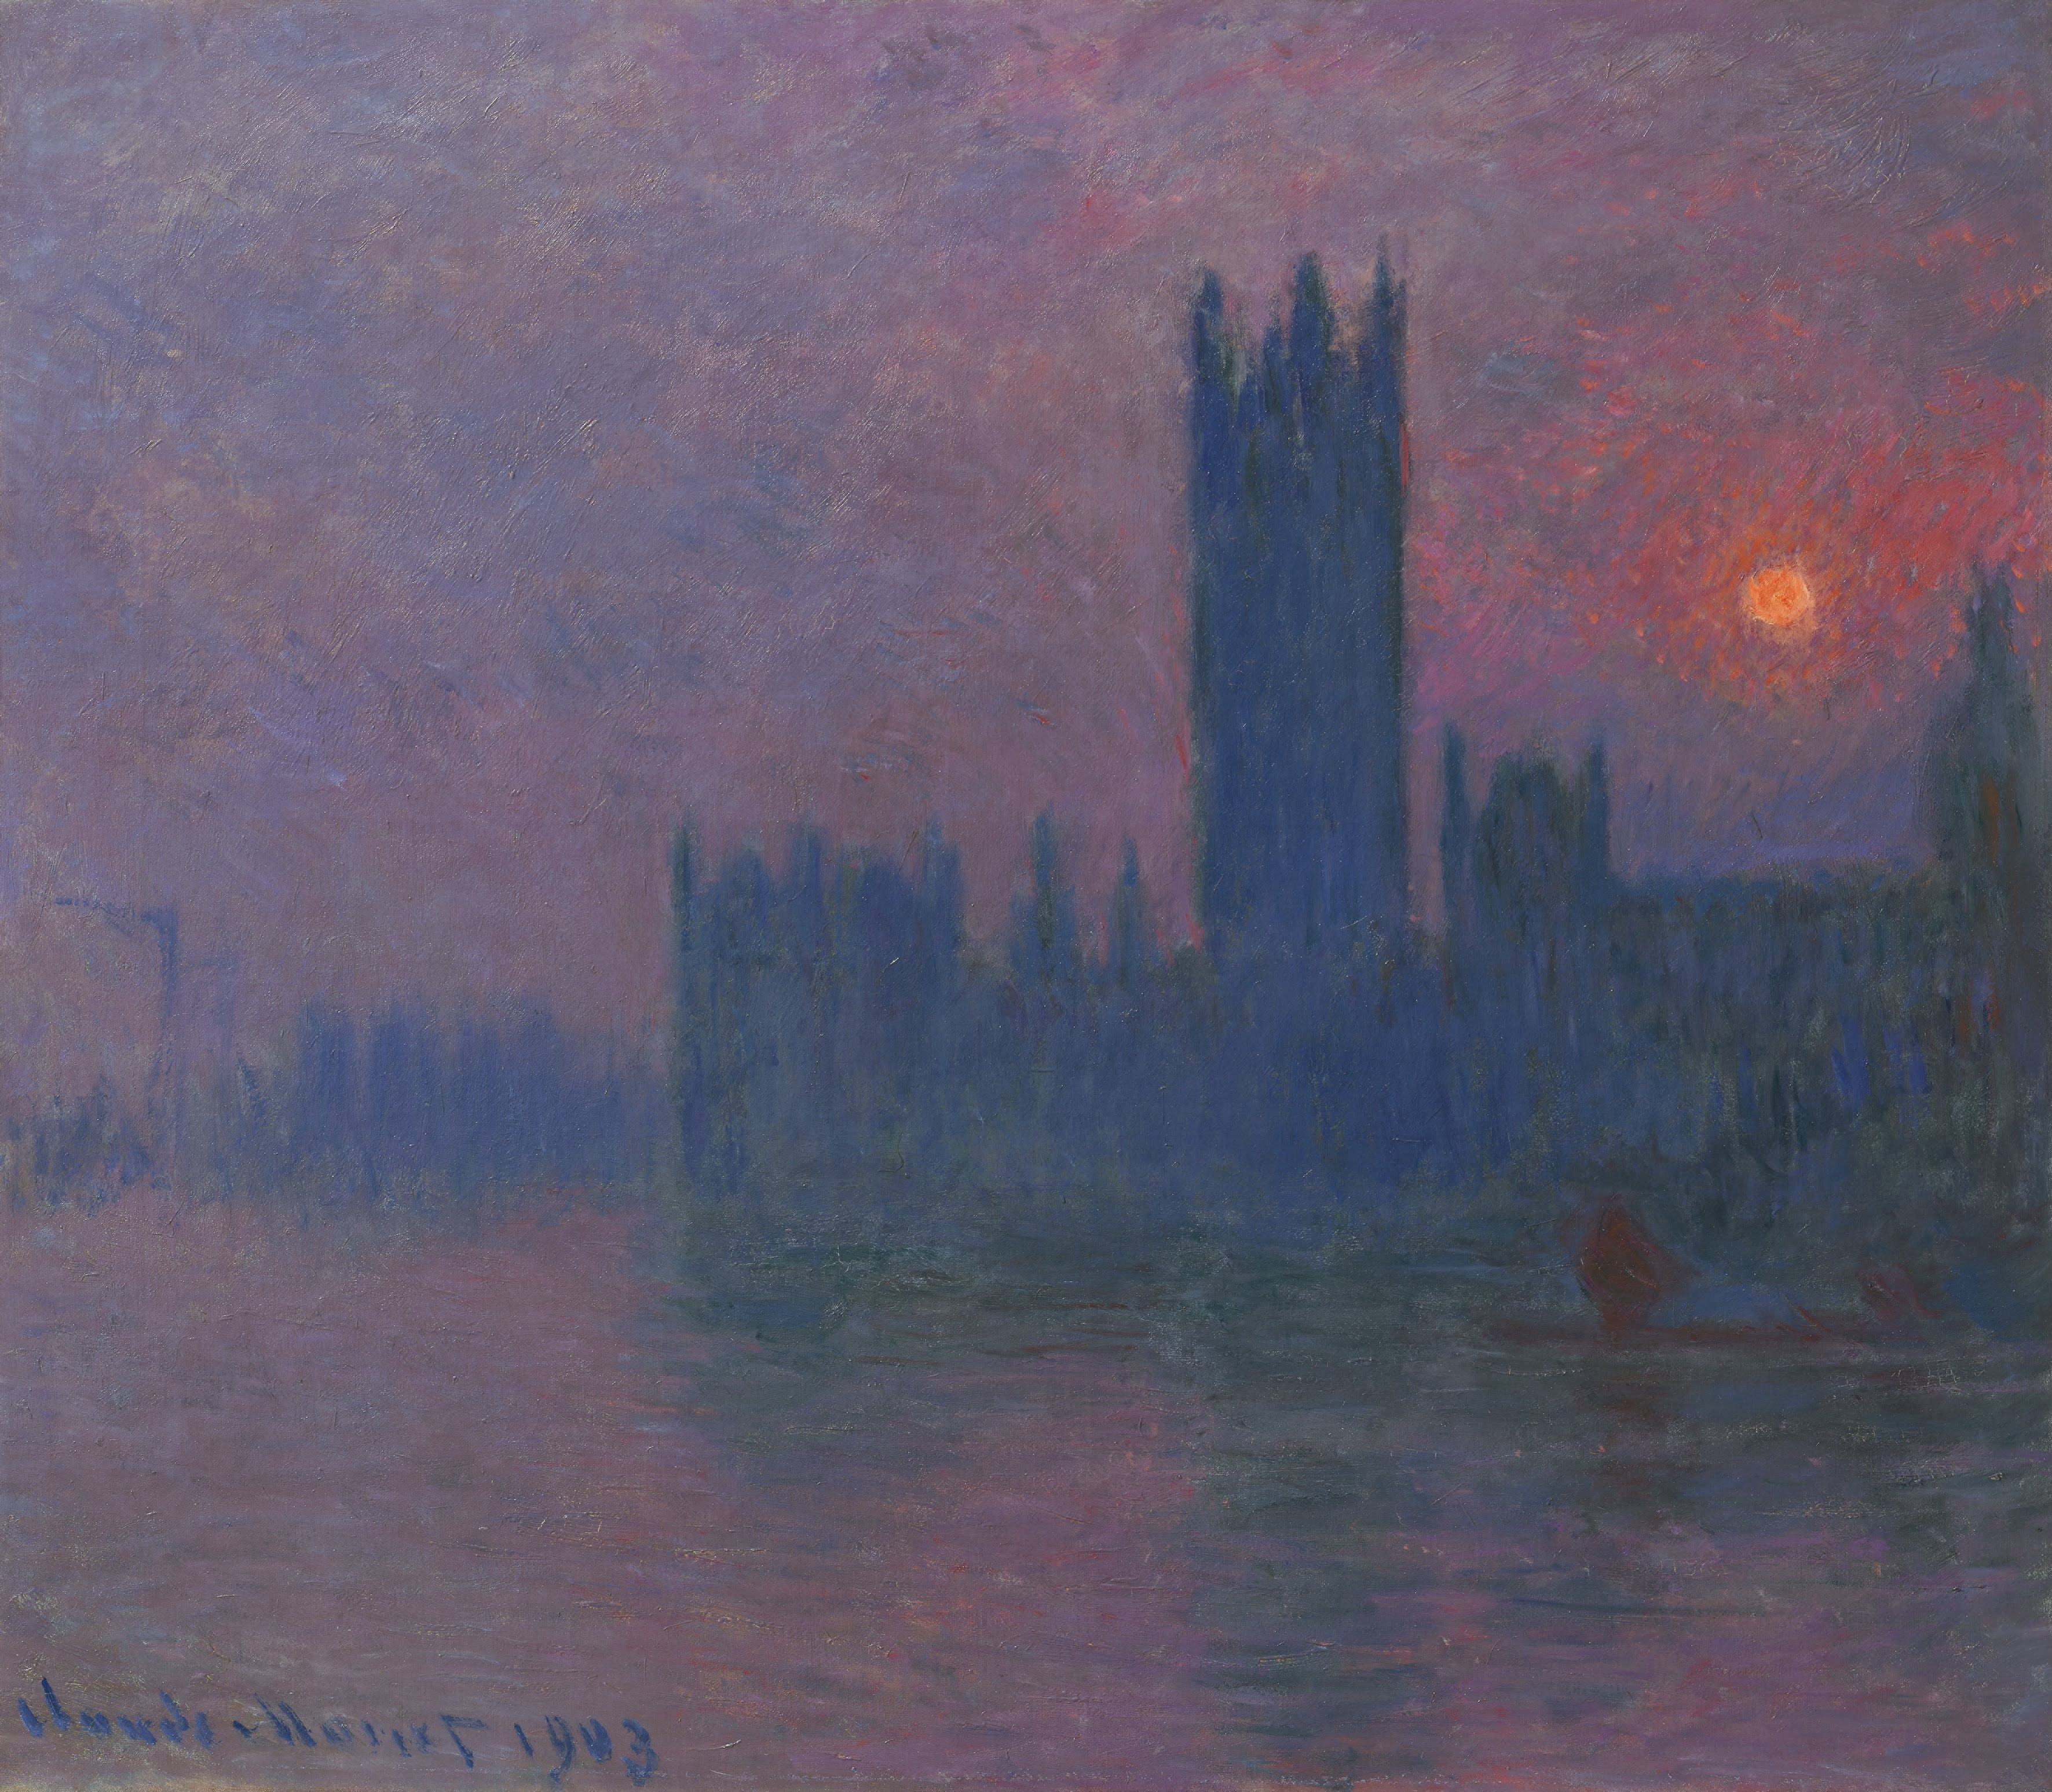
\includegraphics[width=1\linewidth]{london.png}
%   \caption{Claude Monet - Domy parlamentu, zachód słońca (1903)}
% \end{figure}

% Algorytmy kmeans oraz klasteryzacja spektralna radzą sobie średnio z wykrywaniem dominujących kolorów. Nawet jeśli ustawimy k=20, to nie pojawia się kolor słońca (skandal(!)). Testowałem dla różnych metryk, jednak resultaty są kiepskie.

% \begin{figure}[H]
%     \includegraphics[width=0.9\linewidth]{london_km_5.png}
%   \caption{5 dominujących kolorów wg kmeans}
% \end{figure}

% \begin{figure}[H]
%     \includegraphics[width=0.9\linewidth]{london_km_10.png}
%   \caption{10 dominujących kolorów wg kmeans}
% \end{figure}

% \begin{figure}[H]
%     \includegraphics[width=0.9\linewidth]{london_km_20.png}
%   \caption{20 dominujących kolorów wg kmeans}
% \end{figure}

% \begin{figure}[H]
%     \includegraphics[width=0.9\linewidth]{london_spectr_10.png}
%   \caption{10 dominujących kolorów wg klasteryzacji spektralnej}
% \end{figure}



% % wyniki dla kmeans i spektralnego

% Na szczęście klasteryzacja hierarchiczna radzi sobie dobrze:


% \begin{figure}[H]
%     \includegraphics[width=1\linewidth]{london_hier_10.png}
%   \caption{10 dominujących kolorów wg klasteryzacji hierarchicznej, pojedyńcze łączenie}
% \end{figure}


% \begin{figure}[H]
%     \includegraphics[width=1\linewidth]{mona_hier_10.png}
%   \caption{10 dominujących kolorów wg klasteryzacji hierarchicznej, pojedyńcze łączenie}
% \end{figure}


% \begin{figure}[H]
%     \includegraphics[width=1\linewidth]{mondrian_hier_5.png}
%   \caption{5 dominujących kolorów wg klasteryzacji hierarchicznej, pojedyńcze łączenie}
% \end{figure}


% \begin{figure}[H]
%     \includegraphics[width=1\linewidth]{night_hier_16.png}
%   \caption{16 dominujących kolorów wg klasteryzacji hierarchicznej, łączenie warda}
% \end{figure}


% \begin{figure}[H]
%     \includegraphics[width=1\linewidth]{girl_hier_10.png}
%   \caption{10 dominujących kolorów wg klasteryzacji hierarchicznej, łączenie warda}
% \end{figure}


% \begin{figure}[H]
%     \includegraphics[width=1\linewidth]{tank_man_hier_10.png}
%   \caption{10 dominujących kolorów wg klasteryzacji hierarchicznej, łączenie warda}
% \end{figure}

% \begin{figure}[H]
%     \includegraphics[width=1\linewidth]{stanczyk_hier_10.png}
%   \caption{10 dominujących kolorów wg klasteryzacji hierarchicznej, łączenie warda}
% \end{figure}

% \begin{figure}[H]
%     \includegraphics[width=1\linewidth]{afghan_girl_hier_10.png}
%   \caption{10 dominujących kolorów wg klasteryzacji hierarchicznej, łączenie warda}
% \end{figure}




% \begin{figure}[H]
%     \includegraphics[width=1\linewidth]{night_trees.png}
%   \caption{Drzewa hierarchiczne dla różnych metod łączenia: pojedyńcze, centroidalne, średnie, pełne, Warda}
% \end{figure}

% \begin{figure}[H]
%     \includegraphics[width=1\linewidth]{london_trees.png}
%   \caption{Drzewa hierarchiczne dla różnych metod łączenia: pojedyńcze, centroidalne, średnie, pełne, Warda}
% \end{figure}

% \begin{figure}[H]
%     \includegraphics[width=1\linewidth]{girl_trees.png}
%   \caption{Drzewa hierarchiczne dla różnych metod łączenia: pojedyńcze, centroidalne, średnie, pełne, Warda}
% \end{figure}

% \begin{figure}[H]
%     \includegraphics[width=1\linewidth]{tree_tree.png}
%   \caption{Drzewa hierarchiczne dla różnych metod łączenia: pojedyńcze, centroidalne, średnie, pełne, Warda}
% \end{figure}







% \section{Podsumowanie}

% Ciężko jest oceniać wyniki klasteryzacji - używana przeze mnie miara nie zawsze jest dobra. Wydaje mi się jednak, że krzywa błąd klasteryzacji-liczba klastrów może być użytecznym narzędziem do banania 'zgrupowania' danych. Ponad to, przyglądając się drzewom postałym przy klasteryzacji hierarchicznej można dowiedzieć się czegoś o danych. Możnaby też wprowadzić metryki oparte na powstałych drzewach - np.: średnia głębokość liścia, średnia szerokość drzewa, średnia wielkość poddrzewa, etc.. Myślę, że niektóre z nich mogłyby okazać się sensownymi pojęciami w analizie danych. 

% \section{Możliwe dalsze kroki}

% Oto pomysły na dalszą analizę:

% \begin{itemize}
%     \item Wykrycie kilku (np. 8) dominujących kolorów per obraz dla wielu obrazów danego artysty/artystów i zrobienie klasteryzacji na tuplach 8x3=24 wymiarowych (na zbiorach kolorów używanych w danym obrazie). Być może powiedziałoby to coś o stylu danego artysty lub o generalnych tendencjach estetycznych danej epoki.
%     \item Zrobienie programu, który wykrywa dominujące kolory na tapecie i na tej podstawie dobiera kolory terminala i systemowego interfejsu.
%     \item Opracowanie różnych metryk spójności opartych na drzewach hierarchicznych.
% \end{itemize}


\end{document}
